\documentclass[12pt,a4paper]{article}

% --- Page Layout -------------------------------------------------------------
\usepackage[a4paper, margin=0.8in, headheight=14pt]{geometry}

% --- Fonts (XeLaTeX) ---------------------------------------------------------
\usepackage{fontspec}
\usepackage{unicode-math}
\setmainfont{TeX Gyre Pagella}
\setmonofont[Scale=0.88]{TeX Gyre Cursor}
\setmathfont{Latin Modern Math}

% --- Packages ---------------------------------------------------------------
\usepackage{xcolor}
\usepackage{titlesec}
\usepackage{enumitem}
\usepackage{tabularx}
\usepackage{booktabs}
\usepackage{array}
\usepackage{amsmath}
\usepackage{tikz}
\usetikzlibrary{shapes.geometric, arrows.meta, positioning, calc, fit, decorations.pathreplacing}
\usepackage{tcolorbox}
\tcbuselibrary{skins, breakable}
\usepackage{hyperref}
\usepackage{fancyhdr}
\usepackage{graphicx}
\usepackage{microtype}
\hyphenpenalty=10000
\exhyphenpenalty=10000
\sloppy
\usepackage{caption}
\usepackage{setspace}
\usepackage{multirow}
\usepackage{tocloft}

% --- Q&A helper --------------------------------------------------------------
\newcommand{\Q}[1]{\textbf{#1}\par\noindent\ignorespaces}

% --- Colour Palette ----------------------------------------------------------
\definecolor{myred}{RGB}{196,30,58}
\definecolor{mydark}{RGB}{30,30,50}
\definecolor{mygreen}{RGB}{14,120,80}
\definecolor{myteal}{RGB}{0,130,140}
\definecolor{myamber}{RGB}{180,100,0}
\definecolor{mypurple}{RGB}{100,30,160}
\definecolor{mygray}{RGB}{246,247,249}
\definecolor{mgframe}{RGB}{180,185,200}
\definecolor{watermark}{RGB}{145,150,170}
\definecolor{hdrred}{RGB}{250,232,235}
\definecolor{hdrgreen}{RGB}{220,244,233}
\definecolor{hdrteal}{RGB}{220,242,244}
\definecolor{hdramber}{RGB}{253,242,215}
\definecolor{hdrpurple}{RGB}{238,228,255}
\definecolor{hdrgray}{RGB}{238,240,245}
\definecolor{rowalt}{RGB}{250,251,253}

% --- Section Formatting ------------------------------------------------------
\titleformat{\section}
  {\large\bfseries\color{myred}}{\thesection.}{0.5em}{}
  [\vspace{1pt}{\color{myred}\rule{\linewidth}{0.8pt}}]
\titleformat{\subsection}
  {\normalsize\bfseries\color{myteal}}{\thesubsection}{0.5em}{}
\titlespacing*{\section}{0pt}{18pt}{7pt}
\titlespacing*{\subsection}{0pt}{11pt}{4pt}

% --- Paragraph ---------------------------------------------------------------
\setlength{\parindent}{0pt}
\setlength{\parskip}{4pt}

% --- TOC Styling -------------------------------------------------------------
\renewcommand{\cfttoctitlefont}{\large\bfseries\color{myred}}
\renewcommand{\cftaftertoctitle}{\par\noindent{\color{myred}\rule{\linewidth}{0.8pt}}}
\setlength{\cftbeforetoctitleskip}{0pt}
\setlength{\cftaftertoctitleskip}{6pt}
\renewcommand{\cftsecfont}{\normalsize\bfseries\color{mydark}}
\renewcommand{\cftsecpagefont}{\normalsize\bfseries\color{mydark}}
\renewcommand{\cftsecleader}{\cftdotfill{\cftdotsep}}
\setlength{\cftbeforesecskip}{7pt}
\renewcommand{\cftsubsecfont}{\small\color{mydark}}
\renewcommand{\cftsubsecpagefont}{\small\color{mydark}}
\setlength{\cftbeforesubsecskip}{3pt}
\setlength{\cftsubsecindent}{1.4em}

% --- Table helpers -----------------------------------------------------------
\renewcommand{\arraystretch}{1.45}
\setlength{\tabcolsep}{6pt}
\newcolumntype{B}[1]{>{\small\bfseries\raggedright\arraybackslash}m{#1}}
\newcolumntype{Y}{>{\small\raggedright\arraybackslash}X}
\renewcommand{\tabularxcolumn}[1]{m{#1}}

% --- Header / Footer ---------------------------------------------------------
\pagestyle{fancy}
\fancyhf{}
\fancyhead[L]{\small\color{myred}\textbf{BS-CH101}\;\color{mydark}--- Chemistry-I}
\fancyhead[R]{\small\color{myteal}\textbf{Module 4 Notes}}
\fancyfoot[C]{\small\color{mydark}\thepage}
\fancyfoot[R]{\small\color{watermark}\textit{\copyright\ Biraj}}
\renewcommand{\headrulewidth}{0.5pt}
\renewcommand{\footrulewidth}{0.3pt}

% --- Hyperref ---------------------------------------------------------------
\hypersetup{
  colorlinks=true, linkcolor=myteal, urlcolor=myteal,
  pdfauthor={Biraj Sarkar},
  pdftitle={BS-CH101 --- Module 4 Notes}
}

% --- tcolorbox styles --------------------------------------------------------
\tcbset{
  tikzbox/.style={
    colback=mygray, colframe=mgframe, boxrule=0.6pt, arc=4pt,
    left=8pt, right=8pt, top=6pt, bottom=6pt,
    colbacktitle=mgframe, coltitle=mydark,
    fonttitle=\small\bfseries
  },
  defbox/.style={
    colback=hdrgreen, colframe=mygreen, boxrule=0.8pt, arc=4pt,
    left=9pt, right=9pt, top=6pt, bottom=6pt,
    colbacktitle=mygreen, coltitle=white,
    fonttitle=\small\bfseries
  },
  formulabox/.style={
    colback=hdrteal, colframe=myteal, boxrule=0.8pt, arc=4pt,
    left=9pt, right=9pt, top=7pt, bottom=7pt,
    colbacktitle=myteal, coltitle=white,
    fonttitle=\small\bfseries
  },
  examplebox/.style={
    colback=hdramber, colframe=myamber, boxrule=0.8pt, arc=4pt,
    left=9pt, right=9pt, top=6pt, bottom=6pt,
    colbacktitle=myamber, coltitle=white,
    fonttitle=\small\bfseries
  },
  masonbox/.style={
    colback=hdrpurple, colframe=mypurple, boxrule=0.8pt, arc=4pt,
    left=9pt, right=9pt, top=6pt, bottom=6pt,
    colbacktitle=mypurple, coltitle=white,
    fonttitle=\small\bfseries
  },
  exambox/.style={
    colback=hdrpurple, colframe=mypurple, boxrule=1pt, arc=5pt,
    left=10pt, right=10pt, top=8pt, bottom=8pt,
    colbacktitle=mypurple, coltitle=white,
    fonttitle=\bfseries,
    breakable, title after break={\textbf{Frequently Asked / Viva Questions (contd.)}}}
}
\tcbset{breakable}

% --- TikZ styles -------------------------------------------------------------
\tikzset{
  block/.style={rectangle, draw=myteal, fill=hdrteal,
    text width=2.4cm, align=center, minimum height=0.95cm,
    font=\small, rounded corners=3pt, line width=0.7pt},
  redblock/.style={rectangle, draw=myred, fill=hdrred,
    text width=2.4cm, align=center, minimum height=0.95cm,
    font=\small, rounded corners=3pt, line width=0.7pt},
  netnode/.style={rectangle, draw=myteal, fill=hdrteal,
    text width=1.5cm, align=center, minimum height=0.8cm,
    font=\small, rounded corners=3pt, line width=0.7pt},
  sumjunc/.style={circle, draw=myamber, fill=hdramber,
    minimum size=0.62cm, font=\small, line width=0.8pt},
  snode/.style={circle, draw=mypurple, fill=hdrpurple,
    minimum size=0.55cm, font=\footnotesize, line width=0.7pt},
  arrow/.style={-Stealth, thick, color=mydark},
  redarrow/.style={-Stealth, thick, color=myred},
  line/.style={thick, color=mydark}
}

\begin{document}

\begin{center}
  {\LARGE\bfseries\color{myred} BS-CH101 / BS-CH201 --- Chemistry-I}\\[5pt]
  {\normalsize\color{mydark} Semester I \quad$\bullet$\quad 3L:1T:0P \quad$\bullet$\quad 4 Credits}\\[3pt]
  {\normalsize\color{myteal}\textbf{Module 4 Exam Notes: Free Energy and Chemical Equilibria}}\\[3pt]
  {\small\color{mydark} CGEC \;$|$\; B.Tech ECE (2023--27) \;$|$\; \textit{Biraj Sarkar}}
\end{center}
\vspace{2pt}
\noindent{\color{myred}\rule{\linewidth}{1.5pt}}
\vspace{2pt}

\hypersetup{linkcolor=mydark}
\tableofcontents
\hypersetup{linkcolor=myteal}
\newpage
% ===============================================================================
\section{Free Energy and Chemical Equilibria}
% ===============================================================================

\begin{tcolorbox}[defbox]
\textbf{Gibbs free energy} is the thermodynamic function that predicts spontaneity at constant temperature and pressure. A process is spontaneous when $\Delta G<0$.
\end{tcolorbox}

\subsection{First and Second Laws of Thermodynamics}
The first law states conservation of energy. The second law states that total entropy of the universe increases for a spontaneous process.

\begin{tcolorbox}[formulabox, title={Thermodynamic Functions}]
\[
\Delta U=q+w,\qquad \Delta H=\Delta U+\Delta(PV)
\]
\[
\Delta G=\Delta H-T\Delta S
\]
At constant temperature and pressure, $\Delta G<0$ means spontaneous, $\Delta G=0$ means equilibrium, and $\Delta G>0$ means non-spontaneous.
\end{tcolorbox}

\subsection{Entropy and Free Energy Estimation}
Entropy measures dispersal of energy. For a reversible process,
\[
\Delta S=\int\frac{\delta q_{\mathrm{rev}}}{T}
\]
Free energy change combines enthalpy and entropy and is useful because it directly predicts useful work and equilibrium direction.

\subsection{Free Energy and Equilibrium Constant}
For a reaction at non-standard condition,
\[
\Delta G=\Delta G^\circ+RT\ln Q
\]
At equilibrium, $\Delta G=0$ and $Q=K$.

\begin{tcolorbox}[formulabox, title={Relation Between Free Energy and Equilibrium Constant}]
\[
\Delta G^\circ=-RT\ln K=-2.303RT\log K
\]
\end{tcolorbox}

\subsection{Cell Potential and Nernst Equation}
Electrochemical cell work is linked with free energy.

\begin{tcolorbox}[formulabox, title={Electrochemical Free Energy}]
\[
\Delta G=-nFE,\qquad \Delta G^\circ=-nFE^\circ
\]
\[
E=E^\circ-\frac{RT}{nF}\ln Q
\]
At $298\ \mathrm{K}$:
\[
E=E^\circ-\frac{0.0591}{n}\log Q
\]
\end{tcolorbox}

\begin{tcolorbox}[tikzbox, title={Galvanic Cell and Electron Flow}]
\centering
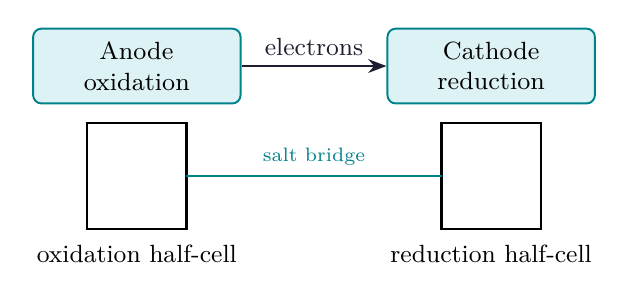
\begin{tikzpicture}[scale=0.9]
  \node[block] (an) at (0,0) {Anode\\oxidation};
  \node[block] (ca) at (5,0) {Cathode\\reduction};
  \draw[arrow] (an) -- node[above,font=\small] {electrons} (ca);
  \draw[thick] (-0.7,-0.8) rectangle (0.7,-2.3);
  \draw[thick] (4.3,-0.8) rectangle (5.7,-2.3);
  \draw[thick,myteal] (0.7,-1.55) -- (4.3,-1.55) node[midway,above,font=\scriptsize] {salt bridge};
  \node[font=\small] at (0,-2.65) {oxidation half-cell};
  \node[font=\small] at (5,-2.65) {reduction half-cell};
\end{tikzpicture}
\end{tcolorbox}

\subsection{Acid-Base, Redox and Solubility Equilibria}
The same free-energy idea applies to acid-base ionization, redox reactions, and precipitation.

\begin{tabularx}{\linewidth}{|B{3.2cm}|Y|Y|}
\hline
\textbf{Equilibrium} & \textbf{Constant} & \textbf{Use} \\
\hline
Acid-base & $K_a$, $K_b$ & pH and strength of acid/base \\
\hline
Redox & $E^\circ$, $K$ & Feasibility of electron transfer \\
\hline
Solubility & $K_{sp}$ & Precipitation and ionic product \\
\hline
\end{tabularx}

\subsection{Water Chemistry, Corrosion and Ellingham Diagram}
Water chemistry includes hardness, alkalinity, pH, and dissolved oxygen. Corrosion is an electrochemical oxidation of metal. Ellingham diagrams plot $\Delta G^\circ$ versus temperature and help choose reducing agents in metallurgy.

\begin{tcolorbox}[tikzbox, title={Ellingham Diagram Concept}]
\centering
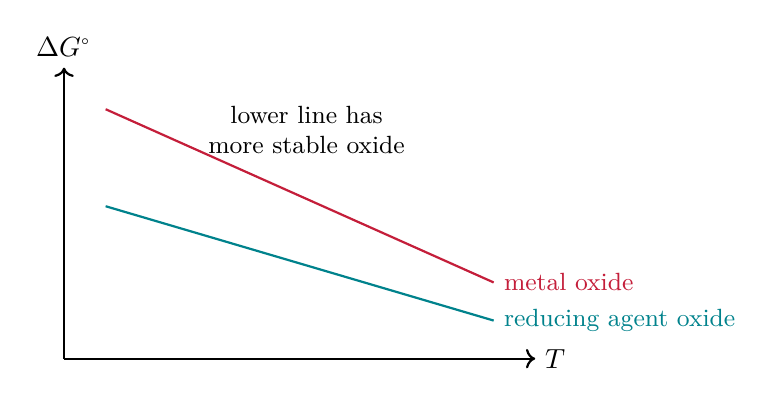
\begin{tikzpicture}[scale=0.88]
  \draw[->, thick] (0,0) -- (6.8,0) node[right] {$T$};
  \draw[->, thick] (0,0) -- (0,4.2) node[above] {$\Delta G^\circ$};
  \draw[myred, thick] (0.6,3.6) -- (6.2,1.1) node[right,font=\small] {metal oxide};
  \draw[myteal, thick] (0.6,2.2) -- (6.2,0.55) node[right,font=\small] {reducing agent oxide};
  \node[font=\small, align=center] at (3.5,3.3) {lower line has\\more stable oxide};
\end{tikzpicture}
\end{tcolorbox}

\begin{tcolorbox}[exambox, title={Exam Points}]
\begin{itemize}[leftmargin=*, itemsep=2pt, topsep=2pt]
  \item Always state sign of $\Delta G$ for spontaneity.
  \item For equilibrium questions, start from $\Delta G=\Delta G^\circ+RT\ln Q$.
  \item For electrochemistry, connect $\Delta G$, $E$, and Nernst equation.
  \item For Ellingham diagrams, lower line means more stable oxide.
\end{itemize}
\end{tcolorbox}

% ===============================================================================
\section{Derivations, Numericals and Engineering Applications}
% ===============================================================================

\subsection{Deriving the Equilibrium Relation}
For any reaction:
\[
\Delta G=\Delta G^\circ+RT\ln Q
\]
At equilibrium, the reaction has no net driving force, so:
\[
\Delta G=0,\qquad Q=K
\]
Therefore:
\[
0=\Delta G^\circ+RT\ln K
\]
\[
\Delta G^\circ=-RT\ln K
\]
Using $\ln K=2.303\log K$:
\[
\Delta G^\circ=-2.303RT\log K
\]

\begin{tcolorbox}[examplebox, title={Solved Example: Equilibrium Constant from Free Energy}]
At $298\ \mathrm{K}$, suppose $\Delta G^\circ=-11.4\ \mathrm{kJ\,mol^{-1}}$.
\[
\log K=\frac{-\Delta G^\circ}{2.303RT}
\]
\[
\log K=\frac{11400}{2.303(8.314)(298)}\approx2.00
\]
\[
K\approx10^2=100
\]
Since $K>1$, products are favoured.
\end{tcolorbox}

\subsection{Entropy Change for Common Processes}
Entropy increases when randomness, volume, or number of gas molecules increases.

\begin{tabularx}{\linewidth}{|B{3.5cm}|Y|Y|}
\hline
\textbf{Process} & \textbf{Entropy change} & \textbf{Reason} \\
\hline
Melting of solid & Positive & Liquid has more molecular freedom \\
\hline
Vaporization & Strongly positive & Gas has much greater randomness \\
\hline
Compression of gas & Negative & Accessible volume decreases \\
\hline
Dissolution of salt & Usually positive & Ions disperse in solution \\
\hline
Crystallization & Negative & Ordered solid forms \\
\hline
\end{tabularx}

\subsection{Nernst Equation Derivation from Free Energy}
Electrical work from a cell is:
\[
\Delta G=-nFE
\]
At standard condition:
\[
\Delta G^\circ=-nFE^\circ
\]
Substitute both in:
\[
\Delta G=\Delta G^\circ+RT\ln Q
\]
\[
-nFE=-nFE^\circ+RT\ln Q
\]
Dividing by $-nF$:
\[
E=E^\circ-\frac{RT}{nF}\ln Q
\]
At $298\ \mathrm{K}$:
\[
E=E^\circ-\frac{0.0591}{n}\log Q
\]

\begin{tcolorbox}[examplebox, title={Solved Example: Cell Potential}]
For a cell with $E^\circ=1.10\ \mathrm{V}$, $n=2$, and $Q=10$:
\[
E=1.10-\frac{0.0591}{2}\log 10
\]
\[
E=1.10-0.02955=1.07045\ \mathrm{V}
\]
\end{tcolorbox}

\subsection{Water Hardness and Boiler Problems}
Hard water contains dissolved calcium and magnesium salts. Temporary hardness is due to bicarbonates; permanent hardness is due to chlorides and sulphates.

\begin{tabularx}{\linewidth}{|B{3.2cm}|Y|Y|}
\hline
\textbf{Problem} & \textbf{Cause} & \textbf{Effect in engineering systems} \\
\hline
Scale formation & Deposition of salts like $\mathrm{CaCO_3}$ & Poor heat transfer and tube overheating \\
\hline
Sludge formation & Loose precipitates in boiler water & Choking and reduced efficiency \\
\hline
Priming & Carryover of water droplets with steam & Wet steam and turbine damage \\
\hline
Foaming & Stable bubbles due to impurities & Irregular boiler operation \\
\hline
Caustic embrittlement & Concentrated alkali in cracks & Boiler metal failure \\
\hline
\end{tabularx}

\subsection{Electrochemical Corrosion Mechanism}
In iron corrosion, anodic and cathodic regions form on the metal surface.

\begin{tcolorbox}[formulabox, title={Rusting Half-Reactions}]
\[
\text{Anode:}\qquad \mathrm{Fe\rightarrow Fe^{2+}+2e^-}
\]
\[
\text{Cathode:}\qquad \mathrm{O_2+2H_2O+4e^-\rightarrow4OH^-}
\]
\[
\mathrm{Fe^{2+}+2OH^-\rightarrow Fe(OH)_2}
\]
Further oxidation gives hydrated ferric oxide, commonly called rust.
\end{tcolorbox}

\subsection{Ellingham Diagram: Reduction Rule}
In metallurgy, a metal oxide can be reduced by an element whose oxide line lies below it in the Ellingham diagram. This means the reducing agent forms a more stable oxide and makes the overall $\Delta G^\circ$ negative.

\begin{tcolorbox}[masonbox, title={Answer-Writing Pattern for Ellingham Problems}]
\begin{enumerate}[leftmargin=*, itemsep=3pt, topsep=2pt]
  \item Identify the oxide to be reduced.
  \item Locate its $\Delta G^\circ$ line at the given temperature.
  \item Find a reducing agent whose oxide line is lower.
  \item State that the net free energy change becomes negative.
\end{enumerate}
\end{tcolorbox}

\subsection{Temperature Dependence of Spontaneity}
The sign of $\Delta G=\Delta H-T\Delta S$ depends on both enthalpy and entropy. This table is a common 5-mark answer.

\begin{tabularx}{\linewidth}{|B{3cm}|Y|Y|}
\hline
\textbf{Case} & \textbf{Sign condition} & \textbf{Spontaneity} \\
\hline
Exothermic, entropy increases & $\Delta H<0,\ \Delta S>0$ & Spontaneous at all temperatures \\
\hline
Endothermic, entropy decreases & $\Delta H>0,\ \Delta S<0$ & Non-spontaneous at all temperatures \\
\hline
Exothermic, entropy decreases & $\Delta H<0,\ \Delta S<0$ & Spontaneous at low temperature \\
\hline
Endothermic, entropy increases & $\Delta H>0,\ \Delta S>0$ & Spontaneous at high temperature \\
\hline
\end{tabularx}

\begin{tcolorbox}[examplebox, title={Solved Example: Temperature of Spontaneity}]
For a reaction, $\Delta H=40\ \mathrm{kJ\,mol^{-1}}$ and $\Delta S=100\ \mathrm{J\,mol^{-1}\,K^{-1}}$.
Convert entropy:
\[
\Delta S=0.100\ \mathrm{kJ\,mol^{-1}\,K^{-1}}
\]
At equilibrium, $\Delta G=0$:
\[
T=\frac{\Delta H}{\Delta S}=\frac{40}{0.100}=400\ \mathrm{K}
\]
Since both $\Delta H$ and $\Delta S$ are positive, the reaction is spontaneous above $400\ \mathrm{K}$.
\end{tcolorbox}

\subsection{pH, Acid Dissociation and Buffer Idea}
For a weak acid:
\[
\mathrm{HA\rightleftharpoons H^+ + A^-}
\]
\[
K_a=\frac{[\mathrm{H^+}][\mathrm{A^-}]}{[\mathrm{HA}]}
\]
For a buffer made of weak acid and its salt:
\[
\mathrm{pH}=pK_a+\log\frac{[\mathrm{salt}]}{[\mathrm{acid}]}
\]

\begin{tcolorbox}[examplebox, title={Solved Example: Buffer pH}]
If $pK_a=4.75$, $[\mathrm{salt}]=0.20\ \mathrm{M}$ and $[\mathrm{acid}]=0.10\ \mathrm{M}$:
\[
\mathrm{pH}=4.75+\log\frac{0.20}{0.10}
\]
\[
\mathrm{pH}=4.75+\log2=4.75+0.301=5.051
\]
\end{tcolorbox}

\subsection{Solubility Product and Common Ion Effect}
For a sparingly soluble salt $\mathrm{AB}$:
\[
\mathrm{AB(s)\rightleftharpoons A^+ + B^-}
\]
\[
K_{sp}=[\mathrm{A^+}][\mathrm{B^-}]
\]
Precipitation occurs when ionic product exceeds $K_{sp}$.

\begin{tabularx}{\linewidth}{|B{3.2cm}|Y|Y|}
\hline
\textbf{Condition} & \textbf{Meaning} & \textbf{Observation} \\
\hline
Ionic product $<K_{sp}$ & Unsaturated solution & No precipitation \\
\hline
Ionic product $=K_{sp}$ & Saturated solution & Equilibrium \\
\hline
Ionic product $>K_{sp}$ & Supersaturated with respect to salt & Precipitation occurs \\
\hline
\end{tabularx}

\subsection{Corrosion Prevention Methods}
Corrosion can be reduced by blocking contact with environment or by making the metal cathodic.

\begin{tabularx}{\linewidth}{|B{3.2cm}|Y|Y|}
\hline
\textbf{Method} & \textbf{Principle} & \textbf{Example} \\
\hline
Painting / coating & Barrier between metal and environment & Paint, oil, polymer coating \\
\hline
Galvanization & Zinc corrodes sacrificially before iron & Zn-coated iron sheets \\
\hline
Cathodic protection & Metal to be protected is made cathode & Pipelines, ship hulls \\
\hline
Alloying & Forms corrosion-resistant surface film & Stainless steel \\
\hline
Inhibitors & Reduce anodic or cathodic reaction rate & Boiler-water additives \\
\hline
\end{tabularx}

\begin{tcolorbox}[masonbox, title={Previous-Year Style Questions}]
\begin{enumerate}[leftmargin=*, itemsep=4pt, topsep=2pt]
  \item Derive $\Delta G^\circ=-RT\ln K$ and explain its significance.
  \item Derive Nernst equation and solve a cell-potential numerical.
  \item Explain water hardness, scale formation and boiler troubles.
  \item Describe electrochemical corrosion of iron and prevention methods.
  \item Explain Ellingham diagram and its use in metallurgy.
\end{enumerate}
\end{tcolorbox}
\newpage
\begin{center}
  {\large\bfseries\color{myred} Quick Revision --- Module 4}\\[3pt]
  {\small\color{mydark} Free Energy and Chemical Equilibria $|$ BS-CH101}
\end{center}
\noindent{\color{myred}\rule{\linewidth}{1.2pt}}
\vspace{4pt}

\begin{tcolorbox}[formulabox, title={Key Formulas at a Glance}]
\begin{tabularx}{\linewidth}{|B{4.0cm}|Y|}
\hline
\textbf{Formula / Rule} & \textbf{Meaning} \\
\hline
$\Delta U=q+w$ & First law of thermodynamics. \\
\hline
$\Delta G=\Delta H-T\Delta S$ & Gibbs free energy relation. \\
\hline
$\Delta G=\Delta G^\circ+RT\ln Q$ & Free energy at non-standard condition. \\
\hline
$\Delta G^\circ=-RT\ln K$ & Relation between free energy and equilibrium constant. \\
\hline
$\Delta G=-nFE$ & Cell free energy and cell potential. \\
\hline
$E=E^\circ-\displaystyle\frac{RT}{nF}\ln Q$ & Nernst equation. \\
\hline
$K_{sp}=[\mathrm{M}^{m+}]^n[\mathrm{X}^{n-}]^m$ & Solubility product expression. \\
\hline
\end{tabularx}
\end{tcolorbox}

\begin{tcolorbox}[defbox, title={One-Line Definitions}]
\begin{itemize}[leftmargin=*, itemsep=2pt, topsep=2pt]
  \item \textbf{Entropy:} Measure of energy dispersal or randomness.
  \item \textbf{Gibbs free energy:} Energy available for useful work at constant temperature and pressure.
  \item \textbf{Equilibrium constant:} Ratio of product and reactant activities at equilibrium.
  \item \textbf{Nernst equation:} Relation between electrode potential and concentration.
  \item \textbf{Corrosion:} Electrochemical deterioration of a metal.
  \item \textbf{Ellingham diagram:} Plot of $\Delta G^\circ$ for oxide formation versus temperature.
\end{itemize}
\end{tcolorbox}

\begin{tcolorbox}[exambox, title={Frequently Asked / Viva Questions}]
\begin{enumerate}[topsep=0pt, label=\textbf{Q\arabic*.}, itemsep=5pt]
  \item \Q{State the first law of thermodynamics.}
    Energy cannot be created or destroyed; $\Delta U=q+w$.
  \item \Q{What is the criterion of spontaneity using Gibbs free energy?}
    $\Delta G<0$ spontaneous, $\Delta G=0$ equilibrium, $\Delta G>0$ non-spontaneous.
  \item \Q{Write Gibbs free energy equation.}
    $\Delta G=\Delta H-T\Delta S$.
  \item \Q{Relate $\Delta G^\circ$ and equilibrium constant.}
    $\Delta G^\circ=-RT\ln K$.
  \item \Q{How is cell emf related to free energy?}
    $\Delta G=-nFE$.
  \item \Q{State the Nernst equation at 298 K.}
    $E=E^\circ-(0.0591/n)\log Q$.
  \item \Q{What is solubility product?}
    It is the product of ion concentrations in a saturated solution, each raised to stoichiometric power.
  \item \Q{Why does corrosion occur electrochemically?}
    Metal oxidation and reduction of oxygen or hydrogen occur at different surface sites.
  \item \Q{What does an Ellingham diagram show?}
    It shows temperature dependence of standard free energy of oxide formation.
  \item \Q{How is a reducing agent selected from Ellingham diagram?}
    A reducing agent whose oxide line lies below the metal oxide line can reduce that oxide.
\end{enumerate}
\end{tcolorbox}

\begin{tcolorbox}[tikzbox, title={Summary Reference Table}]
\begin{tabularx}{\linewidth}{|B{3cm}|Y|Y|}
\hline
\textbf{Area} & \textbf{Key relation} & \textbf{Exam focus} \\
\hline
Thermodynamics & $\Delta G=\Delta H-T\Delta S$ & Spontaneity and equilibrium \\
\hline
Chemical equilibrium & $\Delta G^\circ=-RT\ln K$ & Direction and extent of reaction \\
\hline
Electrochemistry & $\Delta G=-nFE$ & Cell potential and Nernst equation \\
\hline
Metallurgy & Ellingham diagram & Reduction feasibility \\
\hline
\end{tabularx}
\end{tcolorbox}

\end{document}
